\section{Практична частина}
\setlength{\parindent}{4em}

\begin{center}
  {\textbf{\emph{Отримані результати з теодоліту}}}
\end{center}
\begin{figure}[ht]

\centering

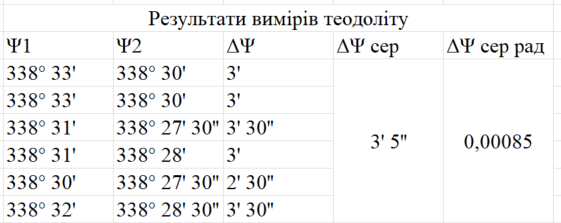
\includegraphics[width=0.55\linewidth]{Pics/Teo.png}


\label{Teo}

\end{figure}
\begin{center}
  {\textbf{\emph{Визначення середньої ширини смуги}}}
\end{center}
\begin{figure}[ht]

\centering

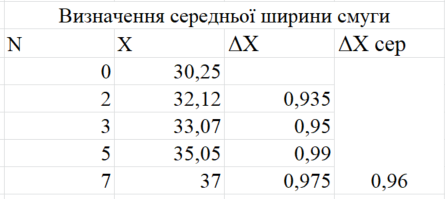
\includegraphics[width=0.55\linewidth]{Pics/width.png}


\label{width}

\end{figure}
\begin{center}
  {\textbf{\emph{Визначення довжини хвилі}}}
\end{center}
\indent Робоча формула:
$$\lambda = \psi \Delta X$$
\begin{figure}[ht]

\centering

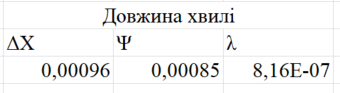
\includegraphics[width=0.4\linewidth]{Pics/lenght.png}


\label{lenght}

\end{figure}

\newpage
\begin{center}
  {\textbf{\emph{Визначення кута біпризми Френеля}}}
\end{center}
\indent Робоча формула:
$$\alpha = \frac{(L+l)\psi}{2l \Delta X}$$
\begin{figure}[ht]

\centering

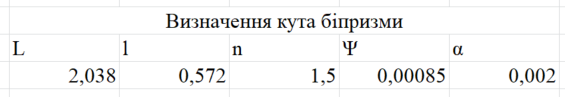
\includegraphics[width=0.6\linewidth]{Pics/alpha.png}


\label{alphs}

\end{figure}
\begin{center}
  {\textbf{\emph{Визначення загальної кількості смуг}}}
\end{center}
\indent Робоча формула:
$$N = L\alpha = \frac{L(L+l)\psi}{2l \Delta X}$$
\begin{figure}[ht]

\centering

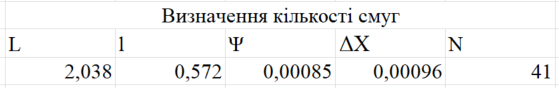
\includegraphics[width=0.6\linewidth]{Pics/count.png}


\label{count}

\end{figure}
\newpage
\subsection{Порівняння отриманих результатів з теоретичними даними}
\indent У ході лабораторної роботи, нами були отримані значення для величин, що ми можемо порівняти з теоретичними:
\begin{enumerate}
  \item $\lambda = 8.16 \cdot 10^{-7}$ нм
  \item $N = 41$ - загальна кількість смужок
\end{enumerate}
Результат, отриманий нами при спостережені смужок в оптичний прилад дає наступні результати: $N_{заг} = 53$. Теоретичне відхилення отриманого нами результату: $\epsilon = \frac{53-41}{53} = 22\%$
З теоретичних данних ми знаемо, що довжина світлової хвилі варіюється від приблизно 700 нм до 400 нм. Таким чином, отриманий нами результат не потрапляє у  теоретичний проміжок. Знайдемо похибку вимірювання для довжини хвилі.\\
